%%%%%%%%%%%%%%%%%%%%%%%%%%%%%%%%%%%%%%%%%%%%%%%%%%%%%%%%%%%%%%%%%%%%%%%%%%%%%%%%
%%                          uAlberta Thesis Template                          %%
%%                                     by                                     %%
%%                               Daniel Aldrich                               %%
%%                               Version: 2.0.0                               %%
%%%%%%%%%%%%%%%%%%%%%%%%%%%%%%%%%%%%%%%%%%%%%%%%%%%%%%%%%%%%%%%%%%%%%%%%%%%%%%%%
%                                                                              %
%       Copyright (c) 2023 Daniel Aldrich                                      %
%                                                                              %
%       Permission is hereby granted, free of charge, to any person            %
%       obtaining a copy of this software and associated documentation         %
%       files (the "Software"), to deal in the Software without                %
%       restriction, including without limitation the rights to use,           %
%       copy, modify, merge, publish, distribute, sublicense, and/or           %
%       sell copies of the Software, and to permit persons to whom the         %
%       Software is furnished to do so, subject to the following               %
%       conditions:                                                            %
%                                                                              %
%       The above copyright notice and this permission notice shall be         %
%       included in all copies or substantial portions of the Software.        %
%                                                                              %
%       THE SOFTWARE IS PROVIDED "AS IS", WITHOUT WARRANTY OF ANY KIND,        %
%       EXPRESS OR IMPLIED, INCLUDING BUT NOT LIMITED TO THE WARRANTIES        %
%       OF MERCHANTABILITY, FITNESS FOR A PARTICULAR PURPOSE AND               %
%       NONINFRINGEMENT. IN NO EVENT SHALL THE AUTHORS OR COPYRIGHT            %
%       HOLDERS BE LIABLE FOR ANY CLAIM, DAMAGES OR OTHER LIABILITY,           %
%       WHETHER IN AN ACTION OF CONTRACT, TORT OR OTHERWISE, ARISING           %
%       FROM, OUT OF OR IN CONNECTION WITH THE SOFTWARE OR THE USE OR          %
%       OTHER DEALINGS IN THE SOFTWARE.                                        %
%                                                                              %
%%%%%%%%%%%%%%%%%%%%%%%%%%%%%%%%%%%%%%%%%%%%%%%%%%%%%%%%%%%%%%%%%%%%%%%%%%%%%%%%
%                                                                              %
%                                   NOTICE                                     %
% This template and class assume a basic understanding of how LaTeX works.     %
%                                                                              %
%%%%%%%%%%%%%%%%%%%%%%%%%%%%%%%%%%%%%%%%%%%%%%%%%%%%%%%%%%%%%%%%%%%%%%%%%%%%%%%%
%                                                                              %
% To use this template start by entering in your information in the fields     %
%     below, and in the file `ualberta.xmpdata'. Next remember to delete the   %
%     auto generated text `\lipsum[##]'.                                       %
%                                                                              %
%%%%%%%%%%%%%%%%%%%%%%%%%%%%%%%%%%%%%%%%%%%%%%%%%%%%%%%%%%%%%%%%%%%%%%%%%%%%%%%%

%LIST OF AVAILABLE THEOREM ENVIRONMENTS
  % For the full list of theorems included please see `includeTheroems.tex'
  %
  % To use:
  % \begin{<theorem name>}
  %     <YOUR TEXT HERE>
  % \end{<theorem name>}

\immediate\write18{makeindex \jobname.nlo -s nomencl.ist -o \jobname.nls}
  % Write command to allow the nomenclature to be generated properly.

\documentclass[pdfa, oneside]{ualberta}
  % OPTIONS FOR ualberta.cls:
  % chapterbib - \printreferences now prints references at the end of a chapter
  % 
  % pdfa - to convert the pdfa to PDF/A format (Required for FGSR Submission)
  % 
  % oneside - Standard for submitting to FGSR.
  % 
  % twoside - If you want to print your thesis double sided like a novel.

%%%%%%%%%%%%%%%%%%%%%%%%%%%%%%%%%%%%%%%%%%%%%%%%%%%%%%%%%%%%%%%%%%%%%%%%%%%%%%%%
%                                FILE LOCATIONS                                %
%%%%%%%%%%%%%%%%%%%%%%%%%%%%%%%%%%%%%%%%%%%%%%%%%%%%%%%%%%%%%%%%%%%%%%%%%%%%%%%%
% LaTeX FILES LOCATION
  \addlatexfiles{./00_LaTeX_Files/}
  \insertlatexfile{includePackages} % LOAD ALL PACKAGES TO BE INCLUDED

% PREFATORY LOCATION
  \addprefatory{./01_Prefatory/}

% CHAPTER LOCATION
  \addchapters{./02_Chapters/}

% BIBLIOGRAPHY LOCATION
  % NOTE: if you add bibliography entries after a compilation, you might notice 
  %   references marked `[0]' to fix this just delete the auxiliary files. (*.aux, *.bbl, ... etc)
  % .  - This folder
  % .. - Up one Folder
  \addbibresource{./03_References/References.bib}

% APPENDICES LOCATION
  \addappendices{./04_Appendices/}

% MEDIA LOCATION
  \addmedia{./99_Inclusions/}
  \addimages{Images/}
  \addtables{Tables/}
  \addcode{Code/}
  \addpdf{PDFs/}

%%%%%%%%%%%%%%%%%%%%%%%%%%%%%%%%%%%%%%%%%%%%%%%%%%%%%%%%%%%%%%%%%%%%%%%%%%%%%%%%
%                         ADD ADDITIONAL RESOURCES                             %
%%%%%%%%%%%%%%%%%%%%%%%%%%%%%%%%%%%%%%%%%%%%%%%%%%%%%%%%%%%%%%%%%%%%%%%%%%%%%%%%
  \insertlatexfile{includeTheorems}
  \insertlatexfile{includeMacros}
  \insertlatexfile{listingCodeFormatting}

%%%%%%%%%%%%%%%%%%%%%%%%%%%%%%%%%%%%%%%%%%%%%%%%%%%%%%%%%%%%%%%%%%%%%%%%%%%%%%%%
%                  TITLE PAGE AND FRONTMATTER INFORMATION                      %
%%%%%%%%%%%%%%%%%%%%%%%%%%%%%%%%%%%%%%%%%%%%%%%%%%%%%%%%%%%%%%%%%%%%%%%%%%%%%%%%
% TITLE PAGE INFO
  \title{Thesis Title}              % Title of your Thesis
  \author{First Middle Last}        % Your Full Name
  \degree{\MSc}                     % \MSc, \PhD, \MA, \MEd, \MBA, \MAc, \MFM, \MN, \LLM, or \MMus
  \specialization{}                 % Leave blank if none
  \department{Example Department}   % Fill in the Department unless you are non-Departmental
  \faculty{}                        % Leave blank unless non-Departmental
  \convocationdate{2023}            % Convocation Year

% DON'T FORGET to edit ualberta.xmpdata with the same metadata for the PDF/A

% ABSTRACT
  \abstracttext{%
	This guide is a comprehensive resource crafted for \University\ students tackling their theses with LaTeX. 
	It is designed to simplify the thesis-writing process by offering a detailed walkthrough of a custom LaTeX template tailored to meet the university's formatting requirements. 
	The guide goes beyond mere template usage, providing step-by-step instructions, tips, and best practices for creating a well-structured thesis that adheres to academic standards.

	It also delves into advanced customization techniques, allowing users to achieve specific stylistic elements and formatting nuances that suit their individual needs. 
	Alongside these, the guide introduces JabRef, a robust reference management tool, and explains how to seamlessly integrate it with LaTeX to streamline citation management. 
	Whether you are a novice or an experienced LaTeX user, this guide equips you with the knowledge and tools necessary to produce a polished, professional thesis. 
	By following its clear and concise instructions, students can confidently navigate the complexities of thesis writing, ensuring their work is both technically sound and perfectly laid out. Test.}

% PREFACE
  \preface{
    \textbf{If you need assistance on writing the preface, ask your supervisor.
    Your supervisor must review and verify the preface before it becomes part of the final version of the thesis.}

    A preface is a mandatory component of a thesis, regardless of thesis format, \underline{when} a thesis contains journal articles authored or co-authored by the student (including an accepted paper that is forthcoming at the time of thesis submission). 
    A preface is \underline{also} a mandatory component when the research conducted for the thesis required ethics approval. 
    A preface remains optional if there is no inclusion of journal articles and/or no need for ethics approval.
    
    When required because a thesis contains journal articles, the preface serves as a place for the student to include a statement indicating his or her contribution to the journal articles, such as the identification and design of the research program, the performance of the various parts of the research (including the collection of data, construction of any necessary apparatus, and the performance of experiments), and the analysis of the research data. 
    If any of the work presented in the thesis has led to any publications (accepted or published), these publications must be listed clearly in the preface with their bibliographical details and an indication as to where in the thesis this work is located (e.g. state in which chapter or chapters). 
    For jointly authored publications, indication must also be given as to the relative contributions of the collaborators and co-authors, and a statement as to the proportion of research and writing conducted by the student. 
    Note that permission may be needed if the co-authors hold the copyright in these publications. 
    If ethics approval was required for the research, a statement to this effect must be included in the preface with the details of the approval that was granted. 
    
    Note that the inclusion of a preface does not excuse a student from failing to acknowledge the contributions of others in the body of the thesis, as per the University's Research and Scholarship Integrity Policy and the Code of Student Behaviour. One would still expect to see footnotes, endnotes or in-text references within the thesis acknowledging the works. Acknowledgements, such as thanks to the supervisor and supervisory committee members, to colleagues, lab mates and friends, and to family, do not appear in the preface. 
    
    \textbf{Examples of several prefaces are given in Appendix B and are also available from the FGSR website.}
}
   
  % Optional
    %\preface{%
      %This thesis is an original work by `Your name here'. No part of this thesis has been previously published.
    %}
    
  % Mandatory due to research ethics approval
    %\preface{
      %This thesis is an original work by `Your name here'. 
      %The research project, of which this thesis is a part, received research ethics approval from the University of Alberta Research Ethics Board, Project Name “TITLE”, No. 12345, DATE.
    %}
    
  % Mandatory due to collaborative work
    %\preface{%
      %Some of the research conducted for this thesis forms part of an international research collaboration, led by Professor R.C. Smith at the University of Hogwarts, with Professor D.R. Brown being the lead collaborator at the University of Alberta. 
      %The technical apparatus referred to in chapter 3 was designed by myself, with the assistance of M.C. White and Professor D.R. Brown. 
      %The data analysis in chapter 4 and concluding analysis in chapter 5 are my original work, as well as the literature review in chapter 2.
      %
      %Chapter 3 of this thesis has been published as J.D. Doe, M.C. Smith, and R.C. Smith, “Theoretical Responses to Rays in the Gamma System,” Journal of Scientific Affairs, vol. 165, issue 3, 459-475. 
      %I was responsible for the data collection and analysis as well as the manuscript composition. 
      %M.C. Smith assisted with the data collection and contributed to manuscript edits. R.C. Smith was the supervisory author and was involved with concept formation and manuscript composition. 
    %}

% DEDICATION
  % Dedications, quotations, poems etc are optional. 
  % Ask your supervisor for advice or views on whether to include such matters in an academic work, with the next component serving as the place to thank people.
	\thesisquote{
		``\lipsum*[14]{}''\\- Author of the Quote}
	\dedication{To...}

% ACKNOWLEDGEMENTS
  \acknowledgementtext{%
	While I would love to acknowledge every individual who has influenced this document, I realize that doing so might mean this document never gets finished.

	I want to extend my deepest gratitude to my friends and family for their unwavering support throughout all my accomplishments.

	A special thank-you goes out to the developers and other \LaTeX\ users who have contributed to the \LaTeX\ community. 
	Without their work, this guide wouldn't exist in its current form.

	I'm also incredibly thankful to everyone who provided feedback and support along the way, including those new to \LaTeX. 
	Your fresh perspectives were invaluable in motivating the transformation of the previous version of this template into a full-fledged class, template, and this newly added guide to writing a thesis, complete with examples of the most requested elements to include.
}


%%%%%%%%%%%%%%%%%%%%%%%%%%%%%%%%%%%%%%%%%%%%%%%%%%%%%%%%%%%%%%%%%%%%%%%%%%%%%%%%
%                  NOMENCLATURE, GLOSSARY, ACRONYMS, ETC                       %
%%%%%%%%%%%%%%%%%%%%%%%%%%%%%%%%%%%%%%%%%%%%%%%%%%%%%%%%%%%%%%%%%%%%%%%%%%%%%%%%

% NOMENCLATURE
  %% Note: Nomenclature is automatically sorted alphabetically
% [A] : Constants
% [B] : Latin
% [C] : Greek
% Use \nomunit{$Value\, Units$} to add the value and units for a defined constant

\nomenclature[A]{$c$}{Speed of light in a vacuum inertial system.\nomunit{$299,792,458\, m/s$}}
\nomenclature[A]{$h$}{Planck constant.\nomunit{$6.62607015E-34\, Js$}}
\nomenclature[B]{$E$}{Elastic Constant (Young's Modulus)}
\nomenclature[B]{$T$}{Torque}
\nomenclature[B]{$a$}{Acceleration}
\nomenclature[B]{$v$}{Velocity}
\nomenclature[B]{$m$}{Mass}
\nomenclature[C]{$\varepsilon$}{Strain}
\nomenclature[C]{$\alpha$}{Primary Angle}

% ACRONYMS (Do NOT include periods at the end)
  %% Note: Acronyms are automatically sorted alphabetically

\addacronym{ROFL}{Rolling on floor laughing}
\addacronym{STFU}{Shut the *swear word!* up}
\addacronym{ICYMI}{In case you missed it}
\addacronym{TL;DR}{Too long, didn't read}
\addacronym{LMK}{Let me know}
\addacronym{NVM}{Nevermind}
\addacronym{TGIF}{Thank goodness it's Friday}
\addacronym{TBH}{To be honest}
\addacronym{TBF}{To be frank}
\addacronym{RN}{Right now}
\addacronym{QOTD}{Quote of the day}
\addacronym{OOTD}{Outfit of the day}
\addacronym{BRB}{Be right back}
\addacronym{BTW}{By the way}
\addacronym{LOL}{Laugh out loud}
\addacronym{TTYL}{Talk to you later}
\addacronym{HMU}{Hit me up}
\addacronym{FWIW}{For what it's worth}
\addacronym{IMO}{In my opinion}
\addacronym{IMHO}{In my humble opinion}
\addacronym{IDK}{I don't know}
\addacronym{TBA}{To be announced}
\addacronym{TBD}{To be decided}

% GLOSSARY (Do NOT include periods at the end)
  %% Note: Glossary is automatically sorted alphabetically

\addterm{Strength (STR)}{The character's physical strength. This effects the potency of melee attacks}
\addterm{Dexterity (DEX)}{Agility and accuracy. This affects ranged attacks and dodging}
\addterm{Constitution (CON)}{Physical resilience. This affects hit points and some physical resistances}
\addterm{Intelligence (INT)}{The ability to process problems and wield certain magic. INT affects the number of skill points received}
\addterm{Wisdom (WIS) }{Common sense and spirituality}
\addterm{Charisma (CHR)}{Social skills and sometimes physical appearance}
\addterm{Good}{Having a respect for life, altruism, and selflessness}
\addterm{Evil}{Wicked and often selfish or oppressive}
\addterm{Lawful}{Abides by a core morality or honor system. Can also be judgmental and close-minded}
\addterm{Chaotic}{Free-spirited and sometimes unpredictable. Can also be reckless or reactionary}
\addterm{Neutral}{A balance between Lawful \& Chaotic or Good \& Evil}
\addterm{Ability Score}{One of six numbers (Strength, Dexterity, Constitution, Intelligence, Wisdom, Charisma) that represent a character's physical and mental attributes}
\addterm{AC (Armor Class)}{A number representing how difficult it is to hit a character in combat}
\addterm{Advantage/Disadvantage}{A mechanic where a player rolls two d20s and takes the higher (advantage) or lower (disadvantage) result}
\addterm{Alignment}{A character's ethical and moral perspective, such as Lawful Good or Chaotic Evil}
\addterm{Arcane}{A type of magic derived from study, such as wizardry}
\addterm{Backstory}{The history and background of a character before the campaign begins}
\addterm{Bonus Action}{An additional action a character can take during their turn, often granted by class features or spells}
\addterm{Cantrip}{A spell that can be cast at will without using a spell slot}
\addterm{Class}{The primary archetype of a character, such as Fighter, Wizard, or Rogue, which determines abilities and progression}
\addterm{Combat}{A structured sequence where characters and enemies take turns performing actions like attacking or casting spells}
\addterm{Concentration}{A mechanic where certain spells require ongoing focus, and taking damage can force a concentration check to maintain the spell}
\addterm{d20}{A 20-sided die, the primary die used in D\&D for most rolls}
\addterm{Damage Types}{One of the thirteen (13) categories of damage: acid, bludgeoning, cold, fire, force, lightning, necrotic, piercing, poison, psychic, radiant, slashing, and thunder}
\addterm{Dungeon Master (DM)}{The person who runs the game, narrates the story, and controls the world and NPCs}
\addterm{Encounter}{Any situation where players must overcome a challenge, such as combat, puzzles, or social interaction}
\addterm{Equipment}{The gear and items a character carries, including weapons, armor, and adventuring tools}
\addterm{Experience Points (XP)}{Points gained from overcoming challenges, used to level up a character}
\addterm{Feat}{A special ability or skill a character can choose instead of an ability score increase at certain levels}
\addterm{Familiar}{A magical creature that assists a spellcaster, often summoned by the spell \textit{Find Familiar}}
\addterm{Flanking}{A tactical position where a character attacks an enemy from the opposite side of an ally, often granting a combat advantage (this rule is optional and varies by DM)}
\addterm{Grapple}{A combat action where a character attempts to grab and restrain an opponent}
\addterm{Group Check}{A mechanic where the success of the party depends on the number of successful rolls among the group}
\addterm{Hit Dice (HD)}{Dice used to determine a character's hit points at each level and for healing during short rests}
\addterm{Hit Points (HP)}{A measure of a character's health, reduced when taking damage}
\addterm{Initiative}{A roll made at the start of combat to determine the order of turns.}
\addterm{Inspiration}{A DM-awarded bonus that allows a player to gain advantage on a roll}
\addterm{Ki}{A resource used by monks to perform special abilities}
\addterm{Level}{A measure of a character's progression, determining access to new abilities, spells, and increased hit points}
\addterm{Long Rest}{A period of downtime (usually 8 hours) where characters recover hit points and spell slots}
\addterm{Metagaming}{Using out-of-game knowledge within the game, often discouraged as it can break immersion}
\addterm{Melee}{Combat at close range, typically involving hand-to-hand or short-ranged weapons}
\addterm{Multiclassing}{The practice of taking levels in more than one class, allowing a character to gain abilities from multiple classes}
\addterm{NPC (Non-Player Character)}{Characters controlled by the DM that players interact with, such as villagers, shopkeepers, or enemies}
\addterm{Opportunity Attack}{A reaction that allows a character to make a melee attack against a creature that moves out of their reach}
\addterm{Party}{The group of player characters (PCs) adventuring together}
\addterm{Perception}{A skill representing a character's ability to notice hidden things, typically rolled as a Wisdom check}
\addterm{Proficiency Bonus}{A bonus added to rolls where a character has proficiency, such as with certain skills, weapons, or saving throws}
\addterm{Quiver}{A container for holding arrows or bolts, typically used by archers and ranged combatants}
\addterm{Ranged Attack}{An attack made with a ranged weapon or spell, targeting an enemy at a distance}
\addterm{Reaction}{An instant response to a trigger, such as casting \textit{Counterspell} or making an opportunity attack}
\addterm{Saving Throw}{A roll made to resist a spell, trap, or other effect}
\addterm{Short Rest}{A brief period of downtime (usually 1 hour) where characters can spend Hit Dice to recover hit points}
\addterm{Skill Check}{A roll made to determine the outcome of an action related to a skill, such as Stealth or Acrobatics}
\addterm{Spell Slot}{A resource that determines how many spells a character can cast at each level}
\addterm{Turn}{A player's time to act during a round of combat, typically consisting of movement, an action, and possibly a bonus action or reaction}
\addterm{Vision Types}{Various levels of sight in D\&D, such as Darkvision, Blindsight, and Truesight}
\addterm{Weapon Proficiency}{Determines which weapons a character can use effectively, adding their proficiency bonus to attack rolls}
\addterm{Wisdom}{An ability score representing a player character's insight, perception, and willpower}
\addterm{XP (Experience Points)}{See Experience Points}



%%%%%%%%%%%%%%%%%%%%%%%%%%%%%%%%%%%%%%%%%%%%%%%%%%%%%%%%%%%%%%%%%%%%%%%%%%%%%%%%
%                              BEGIN DOCUMENT                                  %
%%%%%%%%%%%%%%%%%%%%%%%%%%%%%%%%%%%%%%%%%%%%%%%%%%%%%%%%%%%%%%%%%%%%%%%%%%%%%%%%
\begin{document}

  \maketitle                   % Creates the Title Page
  \makeabstract                % Creates the Abstract Page
  \makepreface                 % Creates the Preface Page
  \makequote                   % Creates the Quote Page
  \makededication              % Creates the Dedication Page
  \acknowledgements            % Creates the Acknowledgements Page

% SET ToC...etc SPACING
  %\singlespacing              % 1.00x Spacing
  \onehalfspacing              % 1.50x Spacing
  %\doublespacing              % 1.75x Spacing
  %\truedoublespacing          % 2.00x Spacing
  %\triplespacing              % 3.00x Spacing
  %\baselineskip #.##em        % #.##x Spacing

  \tableofcontents             % Creates the Table of Contents
  \listoftables                % Creates the List of Tables
  \listoffigures               % Creates the List of Figures
  \listofplates                % Creates the List of Plates (photographs)
  \listofsymbols               % Creates the List of Symbols (Nomenclature)
  \abbreviations               % Creates the List of Acronyms (Abbreviations)
  \glsaddall                   % Required for List of Acronyms and Glossary (DO NOT COMMENT)
  \generateglossary            % Creates the Glossary of Terms


%%%%%%%%%%%%%%%%%%%%%%%%%%%%%%%%%%%%%%%%%%%%%%%%%%%%%%%%%%%%%%%%%%%%%%%%%%%%%%%%
%                           ADD YOUR CONTENT HERE                              %
%%%%%%%%%%%%%%%%%%%%%%%%%%%%%%%%%%%%%%%%%%%%%%%%%%%%%%%%%%%%%%%%%%%%%%%%%%%%%%%%
  \bodyoftext                  % Switches the style of the document to that required for the body

% SET DOCUMENT SPACING
  %\singlespacing              % 1.00x Spacing **Allowed for FOOTNOTES and LONG QUOTES**
  %\onehalfspacing             % 1.50x Spacing **Minimum Spacing for the THESIS BODY**
  %\doublespacing              % 1.75x Spacing
  \truedoublespacing           % 2.00x Spacing **Required for the ABSTRACT**
  %\triplespacing              % 3.00x Spacing
  %\baselineskip #.##em        % #.##x Spacing

% To insert chapters from a separate tex file use the following commands
% \insertchapter automatically looks in the Chapters folder and also
%   appends the file extension (i.e. do NOT include the '.tex')
% 
% \input is the standard way of including a separate tex file
% \chapter{Example Chapter}\label{ch:Example}
  This chapter aims to provide examples how how to structure and create specific components in your thesis document. The very first one is showing a citation, like the one at the end of this sentence \cite{TEST}. The second shows how to create more than one citation and how they are grouped \cite{testone,cite2,cite3,cite4,cite5}.
This sentence shows how a gap in the citations is handled \cite{testone,cite2,cite3,cite5}. 
  \section{Tables}
  
  % L - Left Aligned (Equal Spacing)
  % C - Center Aligned (Equal Spacing)
  % R - Right Aligned (Equal Spacing)
  % l - Left Aligned (Fit to Contents)
  % c - Center Aligned (Fit to Contents)
  % r - Right Aligned (Fit to Contents)
  
  \begin{table}[!htb]
    \caption{This is a basic table}
    \centering
    \begin{tabularx}{0.75\textwidth}{LCR} 
      % Equally spaced cells that are left, center, and reight aligned. 
      % The entire table will be 75% the width of the text.
      \hline
      \textbf{Left Aligned Title} & \textbf{Centered Title} & \textbf{Right Aligned Title} \\\hline
      This is left aligned & This is centered & This is right aligned \\
      This is left aligned & This is centered & This is right aligned \\
      This is left aligned & This is centered & This is right aligned \\
      This is left aligned & This is centered & This is right aligned \\\hline
    \end{tabularx}
    \label{tab:basicTable}
  \end{table}
  
  \begin{table}[!htb]
    \caption{This is a complex table.}
    \centering
    \begin{tabularx}{\textwidth}{lCR}
      % Left most cell is fitted to the content.
      % The center and right columns are equally spaced cells that are center, and reight aligned. 
      % The entire table will be 75% the width of the text.
      \hline
      \multirow{2}{*}{\textbf{This is two row\quad}} & \multicolumn{2}{c}{\textbf{This is two columns}}\\\cline{2-3} % \cline draws a partial line across cells #-#
       & \textbf{Centered Title} & \textbf{Right Aligned Title} \\\hline
      \multirow{2}{*}{This is two row} & This is centered & This is right aligned \\
       & This is centered & This is right aligned \\\cline{1-1}
      \multirow{2}{*}{This is two row} & This is centered & This is right aligned \\
       & This is centered & This is right aligned \\\hline
    \end{tabularx}
    \label{tab:complexTable}
  \end{table}
  
  
  \section{Figures}
  This section will provide examples of how to create figures, and different types of multi/sub-figures. Additionally, if you have many figures in a section and they are bleeding too much into the following sections a \textbackslash{}clearpage command can be issued before the next section. However, note that this will force the next section to begin on a new page. Note that the first ``figure'' is actually a plate; a plate is the proper title associated with a photograph, using the environment `plate' instead of figure and command listofplates will generate everything for you.
  \begin{plate}[!htb]
    \centering
    \includegraphics[width=0.7\textwidth]{example-image}
    \caption{This is an example of a single image plate.}
    \label{fig:singleImage}
  \end{plate}
  
  \begin{figure}[!htb]
    \centering
    \begin{subfigure}{0.45\textwidth}
      \includegraphics[width=\textwidth]{example-image}
      \caption{} % Leave blank for just letter
      \label{fig:doubleImage:a}
    \end{subfigure}
    ~
    \begin{subfigure}{0.45\textwidth}
      \includegraphics[width=\textwidth]{example-image}
      \caption{} % Leave blank for just letter
      \label{fig:doubleImage:b}
    \end{subfigure}
    \caption{This is an example of a double image figure.}
    \label{fig:doubleImage}
  \end{figure}
  
  \begin{figure}[!htb]
    \centering
    \hspace*{\fill}% Adds space to left of top image (prevents two images from going to top)
    \begin{subfigure}{0.45\textwidth}
      \includegraphics[width=\textwidth]{example-image}
      \caption{} % Leave blank for just letter
      \label{fig:tripleImage:a}
    \end{subfigure}
    \hspace*{\fill} % Adds space to right of top image (prevents two images from going to top)
    \par\vspace{1em}% Adds space between upper and lower images
    \begin{subfigure}{0.45\textwidth}
      \includegraphics[width=\textwidth]{example-image}
      \caption{} % Leave blank for just letter
      \label{fig:tripleImage:b}
    \end{subfigure}
    ~ % Adds space between the two lower figures
    \begin{subfigure}{0.45\textwidth}
      \includegraphics[width=\textwidth]{example-image}
      \caption{} % Leave blank for just letter
      \label{fig:tripleImage:c}
    \end{subfigure}
    \caption{This is an example of a triple image figure.}
    \label{fig:tripleImage}
  \end{figure}
  
  \begin{figure}[!htb]
    \centering
    \hspace*{\fill}% Adds space to left of top image (prevents two images from going to top)
    \begin{subfigure}{0.90\textwidth+1em} % 0.9 = 0.45 + 0.45, and 1em is the width of ~
      \includegraphics[width=\textwidth]{example-image}
      \caption{} % Leave blank for just letter
      \label{fig:tripleImage:a}
    \end{subfigure}
    \hspace*{\fill} % Adds space to right of top image (prevents two images from going to top)
    \par\vspace{1em}% Adds space between upper and lower images
    \begin{subfigure}{0.45\textwidth}
      \includegraphics[width=\textwidth]{example-image}
      \caption{} % Leave blank for just letter
      \label{fig:tripleImage:b}
    \end{subfigure}
    ~ % Adds space between the two lower figures
    \begin{subfigure}{0.45\textwidth}
      \includegraphics[width=\textwidth]{example-image}
      \caption{} % Leave blank for just letter
      \label{fig:tripleImage:c}
    \end{subfigure}
    \caption{This is a second example of a triple image figure.}
    \label{fig:tripleImage}
  \end{figure}
  
  \begin{figure}[!htb]
    \centering
    \begin{subfigure}{0.45\textwidth}
      \includegraphics[width=\textwidth]{example-image}
      \caption{} % Leave blank for just letter
      \label{fig:quadImage:a}
    \end{subfigure}
    ~ % Adds space between the two top figures
    \begin{subfigure}{0.45\textwidth}
      \includegraphics[width=\textwidth]{example-image}
      \caption{} % Leave blank for just letter
      \label{fig:quadImage:b}
    \end{subfigure}
    \par\vspace{1em} % Adds space between upper and lower images
    \begin{subfigure}{0.45\textwidth}
      \includegraphics[width=\textwidth]{example-image}
      \caption{} % Leave blank for just letter
      \label{fig:quadImage:c}
    \end{subfigure}
    ~ % Adds space between the two lower figures
    \begin{subfigure}{0.45\textwidth}
      \includegraphics[width=\textwidth]{example-image}
      \caption{} % Leave blank for just letter
      \label{fig:quadImage:d}
    \end{subfigure}
    \caption{This is an example of a quad image figure.}
    \label{fig:quadImage}
  \end{figure}
  
  \clearpage % forces the remaining images (floats to be placed)
  \section{Equations}
  The following equation has no referencing number:
  \nonumeq{E = & m\ c^2}
  
  \Cref{eq:quickEq} has a reference to it though. Or for more control the source for \Cref{eq:quickEq} can be written out fully as it was for \Cref{eq:quickEq2}.
  
  \numeq{pi = & 3.1415...}{eq:quickEq} % shorthand for the following way of writing equations.
  \begin{align}\label{eq:quickEq2}
    e = & 2.7183...
  \end{align}
  
  If you have multiple equations that you want arranged very neatly, use the align environment and you can assign individual equations numbers as shown in \Cref{eq:multiref:a,eq:multiref:b,eq:multiref:c}.
  \begin{align}%Note: Alignment happens at the "=" character
    \label{eq:multiref:a} Equation1 = & 1 + 1\\
    \label{eq:multiref:b} Equation2 = & 2 + 2\\
    \label{eq:multiref:c} Equation3 = & 3 + 3
  \end{align}
  
  
  
  \printreferences % Add a Reference Section to the end of the Chapter.

\lstset{style=LaTeXStyle} %NOTE This line can be removed as it is only for this demo.

\insertchapter{01_Introduction}
\insertchapter{02_Getting_Started}
\insertchapter{03_Document_Structure}
\insertchapter{04_Figures_Tables}
\insertchapter{05_Mathematical_Equations}
\insertchapter{06_Citations_And_References}
\insertchapter{07_Advanced_Topics_And_Packages}

% How to use the Recommended Softwares
\insertchapter{03_JabRef}



%\insertchapter{02_Example_Chapter}
%\insertchapter{0X_Background}
%\insertchapter{0X_Paper_1}
%\insertchapter{0X_Paper_2}
%\insertchapter{0X_Conclusions_Recommendations_and_Future_Work}


%%%%%%%%%%%%%%%%%%%%%%%%%%%%%%%%%%%%%%%%%%%%%%%%%%%%%%%%%%%%%%%%%%%%%%%%%%%%%%%%
%                                 BIBLIOGRAPHY                                 %
%%%%%%%%%%%%%%%%%%%%%%%%%%%%%%%%%%%%%%%%%%%%%%%%%%%%%%%%%%%%%%%%%%%%%%%%%%%%%%%%

% These two lines make sure that the bibliography starts on a new page.
  \bigskip 
  \clearpage

% SET BIBLIOGRAPHY SPACING
  \singlespacing                % 1.00x Spacing
  %\onehalfspacing              % 1.50x Spacing
  %\doublespacing               % 1.75x Spacing
  %\truedoublespacing           % 2.00x Spacing
  %\triplespacing               % 3.00x Spacing
  %\baselineskip #.##em         % #.##x Spacing
 
%  \nocite{*}  % Uncomment if you have a bibliography with works read but not cited
  \printbibliography[heading=bibintoc]
  \bigskip


%%%%%%%%%%%%%%%%%%%%%%%%%%%%%%%%%%%%%%%%%%%%%%%%%%%%%%%%%%%%%%%%%%%%%%%%%%%%%%%%
%                                  APPENDICES                                  %
%%%%%%%%%%%%%%%%%%%%%%%%%%%%%%%%%%%%%%%%%%%%%%%%%%%%%%%%%%%%%%%%%%%%%%%%%%%%%%%%
\appendix
% SET APPENDIX SPACING
  %\singlespacing               % 1.00x Spacing
  %\onehalfspacing              % 1.50x Spacing
  %\doublespacing               % 1.75x Spacing
  \truedoublespacing            % 2.00x Spacing
  %\triplespacing               % 3.00x Spacing
  %\baselineskip #.##em         % #.##x Spacing

% To insert appendices from a separate tex file use the following commands
% \insertappendix automatically looks in the Appendices folder and also
%   appends the file extension (i.e. do NOT include the '.tex'
%
% \input is the standard way of including a separate tex file
% \chapter{Inserting PDFs}\label{sec:motorSpecs}
% NOTE: the PDFs are inserted at 85% their full size to ensure that they don't overlap any FGSR page formatting required for the headers and footers.
  \section{how to insert a portrait PDF}
    
\includepdf[landscape=false,pages=-,pagecommand={},scale=0.85]{./Appendices/examplePDF}
  \section{How to insert a landscape PDF}
    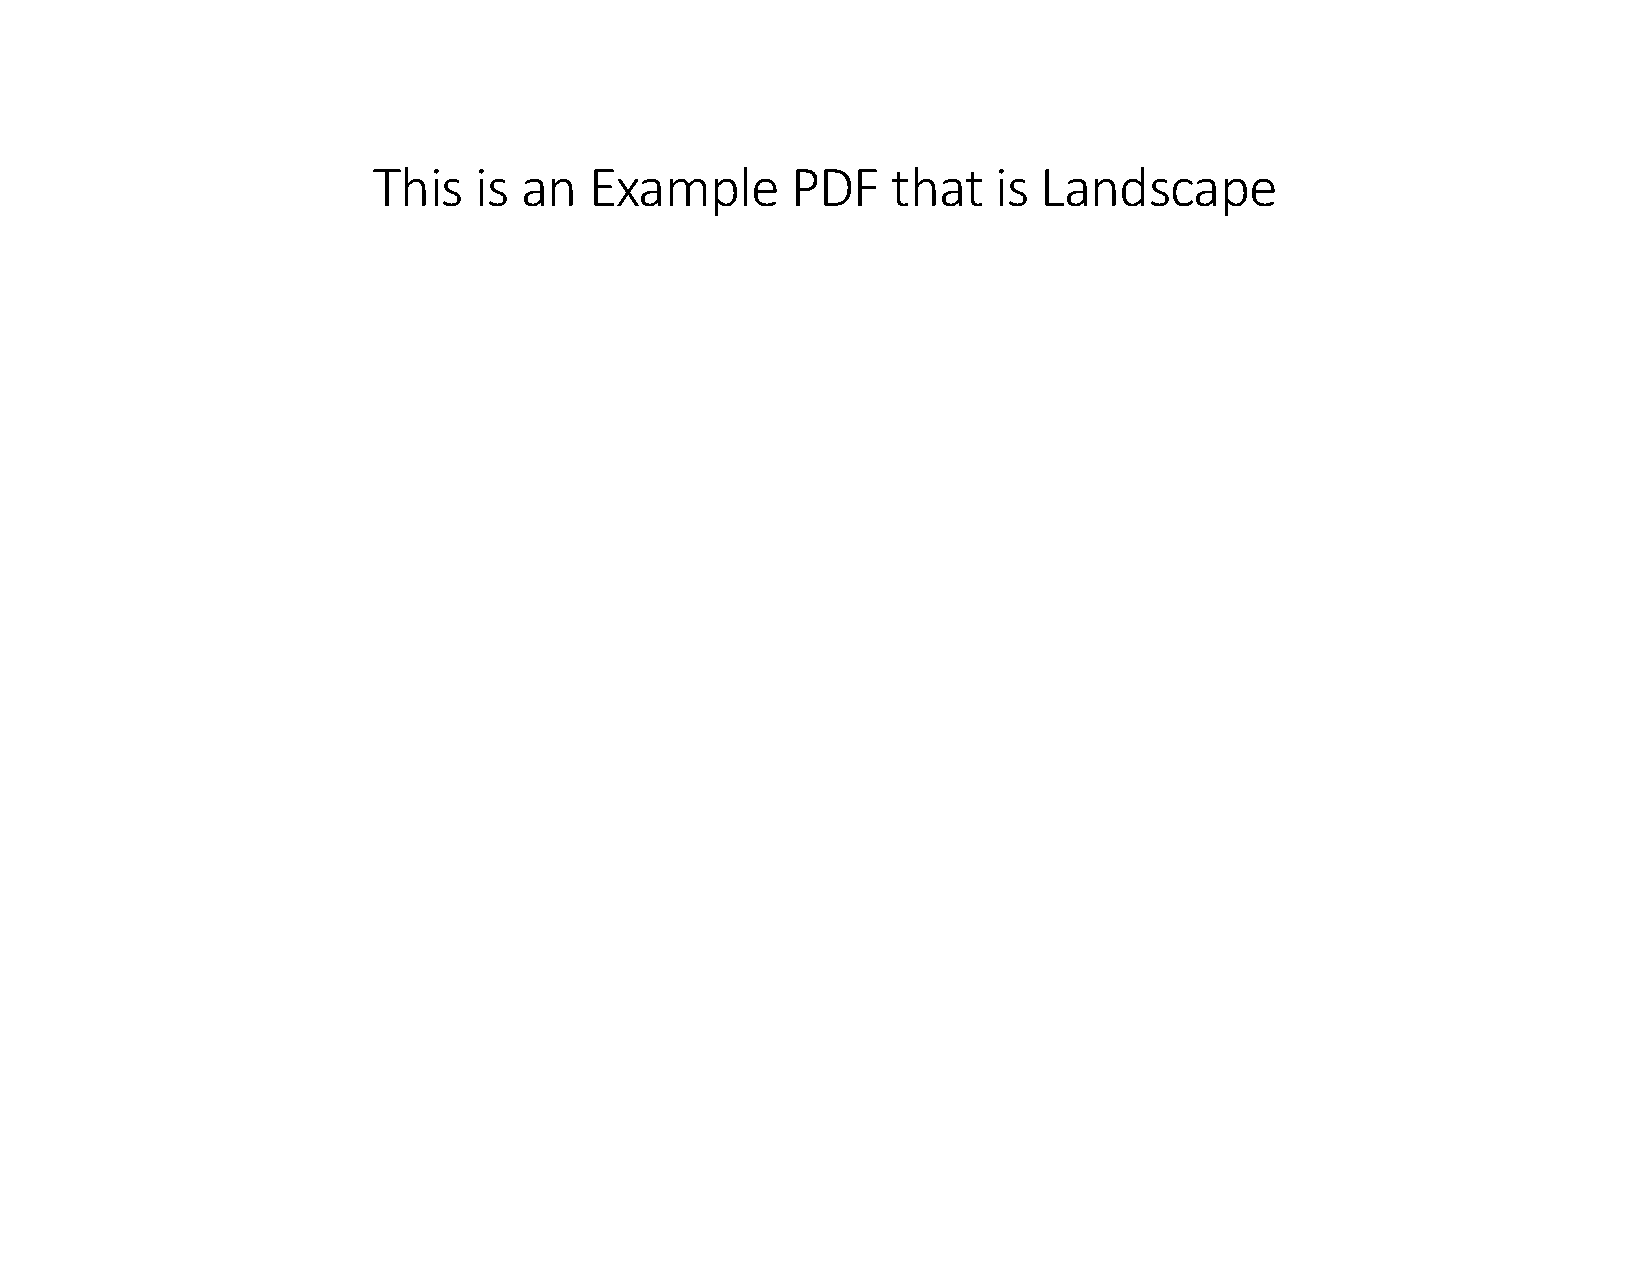
\includepdf[landscape=true,pages=-,pagecommand={},scale=0.85]{./Appendices/landscapePDF}

  \insertappendix{01_Appendix_1}

  \insertappendix{02_Appendix_2}

  \insertappendix{Appendix_Name}

  \insertappendix{PDF_Appendix}

\end{document}
